\section{Usage}

Running Echidna is often as simple as installing it or using the provided Docker image and then typing:

{\scriptsize
\begin{code}
echidna-test MyContract.sol 
\end{code}
}
\noindent In some cases, the contract to test must also be provided, and a configuration file used to modify Echidna's behavior from the default:

{\scriptsize
\begin{code}
echidna-test MyContract.sol --contract Mine--config mc.yaml 
\end{code}
}

\noindent  Echidna can also be called on a directory argument, for contracts that are compiled with the Truffle framework:

{\scriptsize
\begin{code}
echidna-test . --contract TEST
\end{code}
}

\begin{figure}
  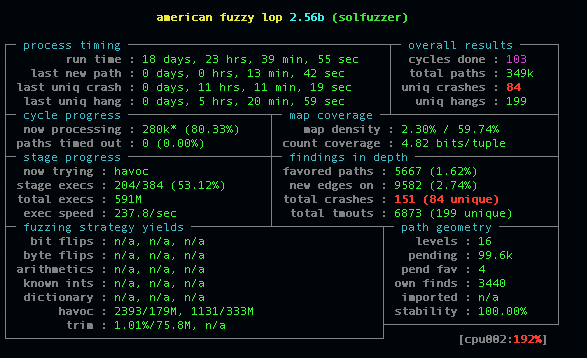
\includegraphics[width=0.9\columnwidth]{echidna.png}
  \caption{The Echidna dashboard.}
  \label{fig:dash}
\end{figure}

\noindent By default, Echidna uses a dashboard output similar to AFL's (Figure \ref{fig:dash}), but a config file can change this to plaintext or JSON output.  The config file also controls various properties of test generation, such as the maximum length of generated transaction sequences, the frequency with which mined constants are used, whether coverage-driven feedback is applied, whether maximum gas usage is computed, and any functions to blacklist from testing.  